\documentclass[11pt,a4paper]{article}
\usepackage[T1]{fontenc}
\usepackage[utf8]{inputenc}
\usepackage{lmodern}
\usepackage{textcomp}
\usepackage[left=1.8cm,right=1.8cm,top=2.3cm,bottom=2.2cm,headheight=14pt,headsep=8pt]{geometry}
\usepackage{multicol}
\usepackage{xcolor}
\usepackage{fancyhdr}
\usepackage{graphicx}
\usepackage{array}
\usepackage{amsmath,amssymb}
\usepackage{setspace}
\usepackage{longtable}
\graphicspath{{../}}
\definecolor{ygreen}{RGB}{46,139,87}
\renewcommand{\normalsize}{\fontsize{10.9}{13.4}\selectfont}
\renewcommand{\familydefault}{\rmdefault}
\setlength{\parindent}{0pt}
\setlength{\columnsep}{0.8cm}
\setlength{\columnseprule}{0.4pt}
\setlength{\multicolsep}{3pt plus 1pt minus 1pt}
\renewcommand{\textsubscript}[1]{\ensuremath{_{\text{\fontsize{8}{8}\selectfont #1}}}}
\renewcommand{\textsuperscript}[1]{\ensuremath{^{\text{\fontsize{8}{8}\selectfont #1}}}}
\newcommand{\diqqat}[1]{\par\smallskip\noindent\textbf{Diqqat!} #1\par\medskip}
\newcommand{\javob}{\par\smallskip\noindent\textbf{Javob:} \rule[-2pt]{7.5cm}{0.4pt}\par\smallskip\noindent\textbf{Diqqat!} Javobingizni javoblar varaqasiga ko`chirib yozing.\par\medskip}
\pagestyle{fancy}
\fancyhf{}
\renewcommand{\headrulewidth}{0.4pt}
\fancyhead[L]{\textit{Milliy sertifikat 2026. Kimyo}}
\fancyhead[R]{2-variant}
\fancyfoot[L]{\fontsize{8}{9}\selectfont \textcopyright{} Colba maktabi, 2026}
\fancyfoot[C]{\thepage}
\fancypagestyle{first}{\fancyhf{}\renewcommand{\headrulewidth}{0pt}\fancyfoot[L]{\fontsize{8}{9}\selectfont \textcopyright{} Colba maktabi, 2026}\fancyfoot[C]{\thepage}}
\begin{document}
\normalsize
\thispagestyle{first}
\noindent\fcolorbox{ygreen}{white}{\parbox{\dimexpr\linewidth-2\fboxsep-2\fboxrule\relax}{%
\textbf{\fontsize{13}{15}\selectfont Nazorat testi}\ \textit{\fontsize{10}{12}\selectfont $\cdot$ Aralash test $\cdot$ 2-variant}\hfill
\begin{tabular}[t]{@{}r@{}}\textit{Milliy sertifikat 2026. Kimyo}\\ \textbf{\textit{\fontsize{8}{9}\selectfont Vaqt:}} \textit{\fontsize{10}{12}\selectfont 180 daqiqa}\end{tabular}}}
\par\medskip
\noindent\textit{Davriy jadvaldan foydalanish mumkin.}
\par\medskip
\begin{multicols}{2}
\noindent\textbf{1.} Atomida 3 ta energetik pog`ona bo`lgan va tashqi pog`onasida 5 ta elektron bo`lgan elementning yuqori oksidi \textbf{formulasini ko`rsating.}

\noindent A)~\textsl{N\textsubscript{2}O\textsubscript{5}} \hfill B)~\textsl{P\textsubscript{2}O\textsubscript{5}} \hfill C)~\textsl{P\textsubscript{2}O\textsubscript{3}} \hfill D)~\textsl{PO\textsubscript{2}}\par
\vspace{4pt}
\noindent\textbf{2.} \textit{X}\textsuperscript{3+} ionida 10 ta elektron va 14 ta neytron bor. \textit{X} atomining nisbiy atom \textbf{massasini aniqlang.}

\noindent A)~\textsl{26} \hfill B)~\textsl{28} \hfill C)~\textsl{24} \hfill D)~\textsl{27}\par
\vspace{4pt}
\noindent\textbf{3.} 0,2 M sirka kislota eritmasida dissotsilanish darajasi 1\% bo`lsa, eritmadagi vodorod ionlari \textbf{konsentratsiyasini (mol/l) aniqlang.}

\noindent A)~\textsl{0,002} \hfill B)~\textsl{0,2} \hfill C)~\textsl{0,0002} \hfill D)~\textsl{0,02}\par
\vspace{4pt}
\noindent\textbf{4.} Zichligi 1,14 g/ml bo`lgan 20\% li H\textsubscript{2}SO\textsubscript{4} eritmasining molyar \textbf{konsentratsiyasini (mol/l) aniqlang.}

\noindent A)~\textsl{4,66} \hfill B)~\textsl{2,33} \hfill C)~\textsl{1,14} \hfill D)~\textsl{2,0}\par
\vspace{4pt}
\noindent\textbf{5.} Jadvalda ikki tuz eritmasi haqida ma'lumot berilgan:
\begin{center}
\renewcommand{\arraystretch}{1.15}
\begin{tabular}{|c|c|c|}\hline
\textbf{Eritma} & \textbf{Massasi, g} & \textbf{Massa ulushi, \%} \\ \hline
1 & 200 & 15 \\ \hline
2 & 300 & 25 \\ \hline
\end{tabular}
\end{center}
Eritmalar aralashtirilganda hosil bo`lgan eritmaning massa \textbf{ulushini (\%) aniqlang.}

\noindent A)~\textsl{21} \hfill B)~\textsl{20} \hfill C)~\textsl{25} \hfill D)~\textsl{22}\par
\vspace{4pt}
\noindent\textbf{6.} 212,5 g 8\% li AgNO\textsubscript{3} eritmasiga mis plastinka tushirildi va kumush to`liq ajralib chiqquncha ushlab turildi. Plastinka massasi necha gramm ortadi?

\noindent A)~\textsl{7,6} \hfill B)~\textsl{10,8} \hfill C)~\textsl{15,2} \hfill D)~\textsl{3,8}\par
\vspace{4pt}
\noindent\textbf{7.} Grafikda A moddaning (A $\to$ mahsulot) konsentratsiyasi vaqt bo`yicha o`zgarishi ko`rsatilgan.
\begin{center}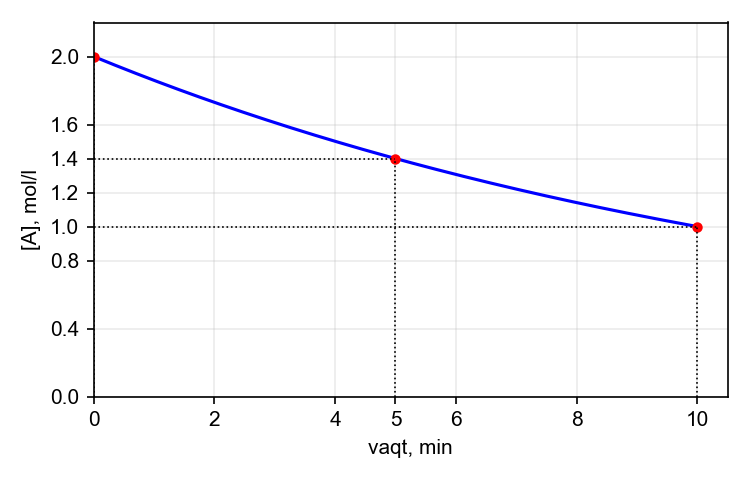
\includegraphics[width=0.86\linewidth]{rasmlar/g_tezlik2.png}\end{center}
Reaksiyaning 5-minutdan 10-minutgacha bo`lgan oraliqdagi o`rtacha tezligini mol/(l$\cdot$min) \textbf{hisoblang.}

\noindent A)~\textsl{0,16} \hfill B)~\textsl{0,8} \hfill C)~\textsl{0,04} \hfill D)~\textsl{0,08}\par
\vspace{4pt}
\noindent\textbf{8.} N\textsubscript{2} + 3H\textsubscript{2} $\rightleftarrows$ 2NH\textsubscript{3} reaksiyada muvozanat qaror topganda [N\textsubscript{2}] = 0,5 mol/l, [H\textsubscript{2}] = 1,5 mol/l, [NH\textsubscript{3}] = 1 mol/l bo`ldi. Vodorodning boshlang`ich \textbf{konsentratsiyasini (mol/l) aniqlang.}

\noindent A)~\textsl{2} \hfill B)~\textsl{4,5} \hfill C)~\textsl{1,5} \hfill D)~\textsl{3}\par
\vspace{4pt}
\noindent\textbf{9.} Tarkibida 3$\cdot$10\textsuperscript{23} ta atom bo`lgan metan (CH\textsubscript{4}) ning \textbf{massasini (g) aniqlang.} (N\textsubscript{A} = 6$\cdot$10\textsuperscript{23})

\noindent A)~\textsl{8} \hfill B)~\textsl{3,2} \hfill C)~\textsl{1,6} \hfill D)~\textsl{0,8}\par
\vspace{4pt}
\noindent\textbf{10.} 27 \textdegree{}C va 2 atm bosimda hajmi 4,92 l bo`lgan gazning massasi 8 g. Gazning molyar \textbf{massasini (g/mol) aniqlang.} (R = 0,082 l$\cdot$atm/(mol$\cdot$K))

\noindent A)~\textsl{20} \hfill B)~\textsl{16} \hfill C)~\textsl{40} \hfill D)~\textsl{32}\par
\vspace{4pt}
\noindent\textbf{11.} 5,4 g metall oksidlanganda 10,2 g oksid hosil bo`ldi. Metallning ekvivalent \textbf{massasini (g/mol) aniqlang.}

\noindent A)~\textsl{18} \hfill B)~\textsl{27} \hfill C)~\textsl{9} \hfill D)~\textsl{12}\par
\vspace{4pt}
\noindent\textbf{12.} 2,5 mol CaCO\textsubscript{3} tarkibidagi kislorod atomlari \textbf{sonini toping.} (N\textsubscript{A} = 6$\cdot$10\textsuperscript{23})

\noindent A)~\textsl{3$\cdot$10\textsuperscript{24}} \hfill B)~\textsl{1,5$\cdot$10\textsuperscript{24}} \hfill C)~\textsl{9$\cdot$10\textsuperscript{24}} \hfill D)~\textsl{4,5$\cdot$10\textsuperscript{24}}\par
\vspace{4pt}
\noindent\textbf{13.} Tarkibida 20\% SO\textsubscript{3} bo`lgan 100 g oleum 400 g suvga qo`shildi. Hosil bo`lgan eritmadagi H\textsubscript{2}SO\textsubscript{4} massa \textbf{ulushini (\%) aniqlang.}

\noindent A)~\textsl{20,9} \hfill B)~\textsl{24,5} \hfill C)~\textsl{19,6} \hfill D)~\textsl{22,4}\par
\vspace{4pt}
\noindent\textbf{14.} 155 g Ca\textsubscript{3}(PO\textsubscript{4})\textsubscript{2} ga mo`l H\textsubscript{2}SO\textsubscript{4} ta'sir ettirilganda 80\% unum bilan hosil bo`lgan fosfat kislota \textbf{massasini (g) aniqlang.}

\noindent A)~\textsl{62,7} \hfill B)~\textsl{78,4} \hfill C)~\textsl{98} \hfill D)~\textsl{49}\par
\vspace{4pt}
\noindent\textbf{15.} NaI va NaCl dan iborat 20 g aralashma orqali mo`l xlor o`tkazilganda aralashma massasi 9,15 g ga kamaydi. Aralashmadagi NaI ning massa \textbf{ulushini (\%) aniqlang.}

\noindent A)~\textsl{60} \hfill B)~\textsl{50} \hfill C)~\textsl{75} \hfill D)~\textsl{80}\par
\vspace{4pt}
\noindent\textbf{16.} 11,5 g natriy suvda eritildi. Hosil bo`lgan eritmadan 0,3 mol CO\textsubscript{2} o`tkazildi. Hosil bo`lgan natriy gidrokarbonat \textbf{massasini (g) aniqlang.}

\noindent A)~\textsl{21,2} \hfill B)~\textsl{8,4} \hfill C)~\textsl{4,2} \hfill D)~\textsl{16,8}\par
\vspace{4pt}
\noindent\textbf{17.} Kalsiy va alyuminiydan iborat 6,7 g aralashma mo`l xlorid kislotada eritilganda 5,6 l (n.sh.) vodorod ajraldi. Aralashmadagi kalsiy \textbf{massasini (g) aniqlang.}

\noindent A)~\textsl{2} \hfill B)~\textsl{4} \hfill C)~\textsl{2,7} \hfill D)~\textsl{5,3}\par
\vspace{4pt}
\noindent\textbf{18.} 9 g Fe(OH)\textsubscript{2} havoda to`liq oksidlanib, Fe(OH)\textsubscript{3} ga aylandi. Hosil bo`lgan Fe(OH)\textsubscript{3} \textbf{massasini (g) aniqlang.}

\noindent A)~\textsl{8} \hfill B)~\textsl{9} \hfill C)~\textsl{12,3} \hfill D)~\textsl{10,7}\par
\vspace{4pt}
\noindent\textbf{19.} 1 l suvda 0,01 mol Ca(HCO\textsubscript{3})\textsubscript{2} va 0,02 mol CaSO\textsubscript{4} erigan. Suv qaynatilgandan keyin qolgan qattiqlikni yo`qotish uchun necha gramm soda (Na\textsubscript{2}CO\textsubscript{3}) kerak?

\noindent A)~\textsl{3,18} \hfill B)~\textsl{2,12} \hfill C)~\textsl{4,24} \hfill D)~\textsl{1,06}\par
\vspace{4pt}
\noindent\textbf{20.} 2,2,3-trimetilpentan molekulasida nechta birlamchi uglerod atomi bor?

\noindent A)~\textsl{6} \hfill B)~\textsl{3} \hfill C)~\textsl{4} \hfill D)~\textsl{5}\par
\vspace{4pt}
\noindent\textbf{21.} Propen va propindan iborat 0,3 mol aralashmani to`liq gidrogenlash uchun 0,5 mol vodorod sarflandi. Aralashmadagi propin \textbf{massasini (g) aniqlang.}

\noindent A)~\textsl{12} \hfill B)~\textsl{4} \hfill C)~\textsl{6} \hfill D)~\textsl{8}\par
\vspace{4pt}
\noindent\textbf{22.} 7,8 g benzoldan 80\% unum bilan nitrobenzol olindi. Hosil bo`lgan nitrobenzol \textbf{massasini (g) aniqlang.}

\noindent A)~\textsl{7,87} \hfill B)~\textsl{9,84} \hfill C)~\textsl{6,15} \hfill D)~\textsl{12,3}\par
\vspace{4pt}
\noindent\textbf{23.} 9,4 g fenol mo`l bromli suv bilan reaksiyaga kirishganda hosil bo`lgan cho`kma \textbf{massasini (g) aniqlang.}

\noindent A)~\textsl{49,6} \hfill B)~\textsl{24,6} \hfill C)~\textsl{33,1} \hfill D)~\textsl{16,5}\par
\vspace{4pt}
\noindent\textbf{24.} Etanal yangi cho`ktirilgan Cu(OH)\textsubscript{2} bilan qizdirilganda 0,2 mol qizil cho`kma (Cu\textsubscript{2}O) hosil bo`ldi. Sarflangan etanal \textbf{massasini (g) aniqlang.}

\noindent A)~\textsl{4,4} \hfill B)~\textsl{6,6} \hfill C)~\textsl{8,8} \hfill D)~\textsl{17,6}\par
\vspace{4pt}
\noindent\textbf{25.} 12 g sirka kislota va 9,2 g etanol aralashmasidan 75\% unum bilan etilatsetat olindi. Efir \textbf{massasini (g) aniqlang.}

\noindent A)~\textsl{13,2} \hfill B)~\textsl{11} \hfill C)~\textsl{17,6} \hfill D)~\textsl{8,8}\par
\vspace{4pt}
\noindent\textbf{26.} 17,6 g etilatsetat mo`l NaOH bilan to`liq gidrolizlandi. Hosil bo`lgan natriy atsetat \textbf{massasini (g) aniqlang.}

\noindent A)~\textsl{18,4} \hfill B)~\textsl{8,2} \hfill C)~\textsl{16,4} \hfill D)~\textsl{12,3}\par
\vspace{4pt}
\noindent\textbf{27.} 162 g kraxmal to`liq gidrolizlanib, hosil bo`lgan glyukoza spirtli bijg`itildi. Hosil bo`lgan etanol \textbf{massasini (g) aniqlang.}

\noindent A)~\textsl{46} \hfill B)~\textsl{184} \hfill C)~\textsl{92} \hfill D)~\textsl{180}\par
\vspace{4pt}
\noindent\textbf{28.} 18,6 g anilin mo`l xlorid kislota bilan reaksiyaga kirishganda hosil bo`lgan tuz \textbf{massasini (g) aniqlang.}

\noindent A)~\textsl{25,9} \hfill B)~\textsl{18,6} \hfill C)~\textsl{12,95} \hfill D)~\textsl{23,4}\par
\vspace{4pt}
\noindent\textbf{29.} Polistirolning molyar massasi 52 000 g/mol bo`lsa, uning polimerlanish \textbf{darajasini aniqlang.}

\noindent A)~\textsl{250} \hfill B)~\textsl{2000} \hfill C)~\textsl{500} \hfill D)~\textsl{1000}\par
\vspace{4pt}
\noindent\textbf{30.} Uch probirkada (\textit{X}, \textit{Y}, \textit{Z}) Mg(NO\textsubscript{3})\textsubscript{2}, Zn(NO\textsubscript{3})\textsubscript{2} va NaNO\textsubscript{3} eritmalari bor. Ularga ketma-ket NaOH eritmasi qo`shildi. Kuzatuvlar jadvalda:
\begin{center}
\renewcommand{\arraystretch}{1.15}
\begin{tabular}{|c|c|c|}\hline
\textbf{Probirka} & \textbf{oz miqdor NaOH} & \textbf{mo`l miqdor NaOH} \\ \hline
\textit{X} & oq cho`kma & cho`kma erimaydi \\ \hline
\textit{Y} & oq cho`kma & cho`kma eriydi \\ \hline
\textit{Z} & o`zgarish yo`q & --- \\ \hline
\end{tabular}
\end{center}
\textit{X}, \textit{Y}, \textit{Z} probirkalardagi \textbf{moddalarni aniqlang.}
\noindent A)~\textsl{\textit{X} -- Mg(NO\textsubscript{3})\textsubscript{2}, \textit{Y} -- NaNO\textsubscript{3}, \textit{Z} -- Zn(NO\textsubscript{3})\textsubscript{2}}\par
\noindent B)~\textsl{\textit{X} -- Mg(NO\textsubscript{3})\textsubscript{2}, \textit{Y} -- Zn(NO\textsubscript{3})\textsubscript{2}, \textit{Z} -- NaNO\textsubscript{3}}\par
\noindent C)~\textsl{\textit{X} -- NaNO\textsubscript{3}, \textit{Y} -- Mg(NO\textsubscript{3})\textsubscript{2}, \textit{Z} -- Zn(NO\textsubscript{3})\textsubscript{2}}\par
\noindent D)~\textsl{\textit{X} -- Zn(NO\textsubscript{3})\textsubscript{2}, \textit{Y} -- Mg(NO\textsubscript{3})\textsubscript{2}, \textit{Z} -- NaNO\textsubscript{3}}\par
\vspace{4pt}
\noindent\textbf{31.} Uch probirkada glyukoza, saxaroza va kraxmal eritmalari bor. Ularni aniqlash uchun qaysi reaktivlardan foydalanish to`g`ri?
\noindent A)~\textsl{FeCl\textsubscript{3} eritmasi, so`ng Ag\textsubscript{2}O (NH\textsubscript{3})}\par
\noindent B)~\textsl{bromli suv, so`ng NaOH}\par
\noindent C)~\textsl{faqat yod eritmasi}\par
\noindent D)~\textsl{yod eritmasi (kraxmal --- ko`k rang), so`ng Cu(OH)\textsubscript{2} qizdirilganda (glyukoza --- qizil cho`kma, saxaroza --- o`zgarmaydi)}\par
\vspace{4pt}
\noindent\textbf{32.} Rasmda gazlarni to`plashning ikki usuli ko`rsatilgan: 1-usul --- suvni siqib chiqarish, 2-usul --- havoni siqib chiqarish (idish og`zi yuqoriga).
\begin{center}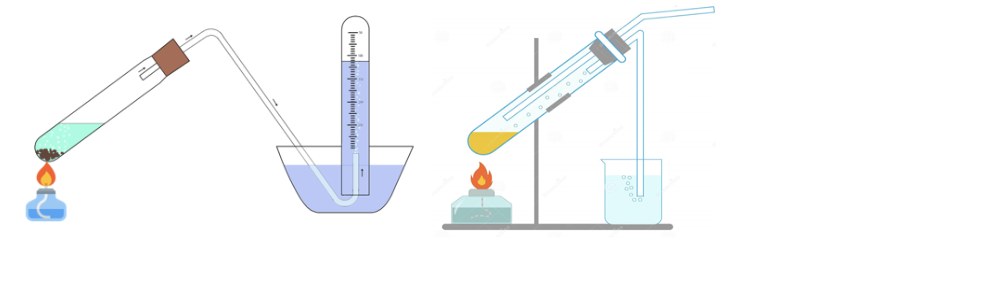
\includegraphics[width=0.86\linewidth]{rasmlar/m_gaz.png}\end{center}
Qaysi gazni rasmdagi ikkala usulda ham to`plab bo`lmaydi?

\noindent A)~\textsl{NH\textsubscript{3}} \hfill B)~\textsl{NO\textsubscript{2}} \hfill C)~\textsl{H\textsubscript{2}} \hfill D)~\textsl{O\textsubscript{2}   ---}\par
\vspace{4pt}
\end{multicols}
\medskip
\noindent\setlength{\fboxsep}{0pt}\fbox{\begin{tabular}{p{0.74\linewidth}|p{0.2\linewidth}}
\parbox[t]{0.72\linewidth}{\vspace{3pt}\textbf{Topshiriqlar (33--35) va javob variant (A--F)larini o`zaro to`g`ri moslashtiring.} 4 l hajmli idishda 2SO\textsubscript{2} + O\textsubscript{2} $\rightleftarrows$ 2SO\textsubscript{3} reaksiyasi o`tkazildi. Moddalar miqdori jadvalda berilgan:
\begin{center}
\renewcommand{\arraystretch}{1.15}
\begin{tabular}{|c|c|c|c|}\hline
\textbf{Modda} & \textbf{SO\textsubscript{2}} & \textbf{O\textsubscript{2}} & \textbf{SO\textsubscript{3}} \\ \hline
Boshlang`ich miqdor, mol & 4 & 3 & 0 \\ \hline
Muvozanatdagi miqdor, mol & --- & --- & 2 \\ \hline
\end{tabular}
\end{center}
\vspace{3pt}} & \parbox[t]{0.19\linewidth}{\vspace{3pt}A~\textsl{0,5}\\[3pt]
B~\textsl{2}\\[3pt]
C~\textsl{50}\\[3pt]
D~\textsl{25}\\[3pt]
E~\textsl{1}\\[3pt]
F~\textsl{14,3}}\\ \hline
\parbox[t]{0.72\linewidth}{\vspace{2pt}\textbf{33. Muvozanat holatida SO\textsubscript{2} ning molyar konsentratsiyasini (mol/l) aniqlang.}\vspace{2pt}} & \\ \hline
\parbox[t]{0.72\linewidth}{\vspace{2pt}\textbf{34. Muvozanat konstantasini (K) aniqlang.}\vspace{2pt}} & \\ \hline
\parbox[t]{0.72\linewidth}{\vspace{2pt}\textbf{35. SO\textsubscript{2} ning necha foizi reaksiyaga kirishgan?}\vspace{2pt}} & 
\end{tabular}}
\par\bigskip
\noindent\textbf{36.} K\textsubscript{2}Cr\textsubscript{2}O\textsubscript{7} + HCl $\to$ CrCl\textsubscript{3} + Cl\textsubscript{2} + KCl + H\textsubscript{2}O reaksiya tenglamasini eng kichik butun sonlarda tenglang va barcha koeffitsiyentlar \textbf{yig`indisini aniqlang.}
\javob
\noindent\textbf{37.} 400 g 10\% li CuSO\textsubscript{4} eritmasi inert elektrodlar yordamida 10 A tok kuchi bilan 3860 s elektroliz qilindi. Elektroliz tugagach, eritmadagi sulfat kislotaning massa \textbf{ulushini (\%) aniqlang} (yaxlitlab, o`ndan birgacha yozing).
\javob
\noindent\textbf{38.} Na\textsubscript{2}CO\textsubscript{3} va NaHCO\textsubscript{3} dan iborat 19 g aralashma doimiy massaga kelguncha qizdirildi, massa 3,1 g ga kamaydi. Dastlabki aralashmadagi Na\textsubscript{2}CO\textsubscript{3} \textbf{massasini (g) aniqlang.}
\javob
\noindent\textbf{39.} Molyar massasi noma'lum bo`lgan to`yingan bir atomli spirtning 6 g massasi natriy bilan to`liq reaksiyaga kirishganda 1,12 l (n.sh.) vodorod ajraldi. Spirtning molyar \textbf{massasini (g/mol) aniqlang.}
\javob
\noindent\textbf{40.} To`yingan bir atomli aldegidning 11,6 g massasi Ag\textsubscript{2}O ning ammiakli eritmasi bilan oksidlanganda 43,2 g kumush ajraldi. Aldegidning molyar \textbf{massasini (g/mol) aniqlang.}
\javob
\par\bigskip\begin{center}\textbf{\fontsize{13}{15}\selectfont YOZMA ISH}\end{center}
\noindent\textbf{41.} \textbf{Topshiriqni bajarish jarayonida barcha reaksiya tenglamalarini yozing. Miqdoriy va arifmetik hisoblashlarni (unga asos bo`lgan usul yoki formulani ko`rsatgan holda) uzviy ketma-ketlikda bajaring.}\par\smallskip
Hajmi 1 l bo`lgan idishga 0,8 mol SO\textsubscript{2} va ma'lum miqdorda O\textsubscript{2} solindi hamda katalizator ishtirokida qizdirildi: 2SO\textsubscript{2} + O\textsubscript{2} $\rightleftarrows$ 2SO\textsubscript{3}. Muvozanat qaror topganda idishda SO\textsubscript{2}, O\textsubscript{2} va SO\textsubscript{3} ning mol nisbati 1 : 1 : 3 bo`ldi.\par
Hosil bo`lgan SO\textsubscript{3} ning hammasi 200 g 49\% li H\textsubscript{2}SO\textsubscript{4} eritmasiga yuttirildi (oleum hosil bo`lmadi, SO\textsubscript{3} to`liq suv bilan reaksiyaga kirishdi). Olingan eritmaga mo`l BaCl\textsubscript{2} eritmasi qo`shildi.\par
\noindent 1)O\textsubscript{2} ning boshlang`ich miqdorini (mol) va muvozanat konstantasini (K) hisoblang.\par
\noindent 2)SO\textsubscript{2} ning necha foizi reaksiyaga kirishgan?\par
\noindent 3)SO\textsubscript{3} yuttirilgandan keyingi eritmada H\textsubscript{2}SO\textsubscript{4} ning massa ulushini (\%) aniqlang.\par
\noindent 4)BaCl\textsubscript{2} qo`shilganda hosil bo`lgan cho`kma massasini (g) toping.\par
\noindent 5)Doimiy haroratda idish hajmi 2 marta kamaytirilsa (v = k$\cdot$[SO\textsubscript{2}]\textsuperscript{2}$\cdot$[O\textsubscript{2}]), to`g`ri reaksiya tezligi necha marta o`zgaradi?\par
\diqqat{Mazkur topshiriq kengaytirilgan javobni talab etib, uning yechilish usuli va shu usul asosidagi barcha hisoblash amallari javoblar varaqasida aks etishi lozim.}
\noindent\textbf{42.} Reaksiya tenglamalarini tugallang va tenglang. Hosil bo`lgan organik moddalarning tuzilish formulalarini yozing va ularni nomlang.\par
\noindent 1)CH\textsubscript{3}--CH\textsubscript{2}--OH + CuO $\xrightarrow{\text{t}}$\par
\noindent 2)CH\textsubscript{3}--CHO + H\textsubscript{2} $\xrightarrow{\text{Ni, t}}$\par
\noindent 3)C\textsubscript{6}H\textsubscript{5}--CH\textsubscript{3} + Cl\textsubscript{2} $\xrightarrow{\text{yorug`lik}}$\par
\noindent 4)CH\textsubscript{3}COOH + C\textsubscript{2}H\textsubscript{5}OH $\rightleftarrows$ (H\textsubscript{2}SO\textsubscript{4})\par
\noindent 5)n CH\textsubscript{2}=CH\textsubscript{2} $\to$\par
\noindent 6)C\textsubscript{6}H\textsubscript{5}NH\textsubscript{2} + HCl $\to$\par
\noindent 7)C\textsubscript{6}H\textsubscript{12}O\textsubscript{6} $\xrightarrow{\text{spirtli bijg`ish}}$\par
\diqqat{Mazkur topshiriq kengaytirilgan javobni talab etib, uning yechilish usuli va shu usul asosidagi barcha hisoblash amallari javoblar varaqasida aks etishi lozim.}
\noindent\textbf{43.} \textbf{Topshiriqni bajarish jarayonida barcha reaksiya tenglamalarini yozing. Miqdoriy va arifmetik hisoblashlarni (unga asos bo`lgan usul yoki formulani ko`rsatgan holda) uzviy ketma-ketlikda bajaring.}\par\smallskip
Uch probirkada XCl\textsubscript{2}, YCl\textsubscript{2} va ZCl\textsubscript{2} tarkibli metall xloridlarining eritmalari bor. Har bir eritmaga reagentlar ta'sir ettirildi, kuzatuvlar jadvalda ("---" belgisi reaksiya bormasligini bildiradi, bo`sh kataklar bo`yicha ma'lumot berilmagan):\par
\begin{center}
\renewcommand{\arraystretch}{1.15}
\begin{tabular}{|c|c|c|c|}\hline
\textbf{Reagent} & \textbf{XCl\textsubscript{2}} & \textbf{YCl\textsubscript{2}} & \textbf{ZCl\textsubscript{2}} \\ \hline
H\textsubscript{2}S & qora cho`kma & --- &  \\ \hline
Na\textsubscript{2}S & qora cho`kma & qora cho`kma & oq cho`kma \\ \hline
NaOH & havorang cho`kma & och yashil cho`kma & oq cho`kma \\ \hline
Zn plastinka & qizil qoplama &  & --- \\ \hline
\end{tabular}
\end{center}
\textit{X}, \textit{Y}, \textit{Z} --- davriy sistemaning to`rtinchi davridagi metallar.\par
\noindent 1)Jadvalda kuzatilgan barcha reaksiyalarning molekulyar tenglamalarini yozing. XCl\textsubscript{2} eritmasiga tushirilgan Zn plastinkada 0,2 mol \textit{X} ajralgan bo`lsa, plastinka massasi qanchaga (g) o`zgargan?\par
\noindent 2)\textit{X}, \textit{Y}, \textit{Z} metallarni aniqlang va tuzlarning formulalarini yozing. XCl\textsubscript{2} tarkibida \textit{X} ning massa ulushi 47,4\% ekanini hisob bilan tasdiqlang.\par
\noindent 3)12,7 g YCl\textsubscript{2} eritmasiga mo`l NaOH qo`shildi, hosil bo`lgan cho`kma havoda to`liq oksidlanguncha qoldirildi. Barcha reaksiya tenglamalarini yozing va oxirgi cho`kma massasini (g) aniqlang.\par
\noindent 4)ZCl\textsubscript{2} ning 13,6 g massasi mo`l NaOH eritmasi bilan reaksiyaga kirishganda hosil bo`lgan kompleks tuz massasini (g) hisoblang (reaksiya tenglamalarini yozing).\par
\diqqat{Mazkur topshiriq kengaytirilgan javobni talab etib, uning yechilish usuli va shu usul asosidagi barcha hisoblash amallari javoblar varaqasida aks etishi lozim.}
\newpage
\noindent\textbf{\fontsize{13}{15}\selectfont Nazorat testi}\ \textit{$\cdot$ 2-variant}\hfill \textbf{Javoblar kaliti}\par\smallskip\hrule\smallskip
\textit{Faqat o`qituvchi uchun.}\par\medskip
\noindent\textbf{1--32-savollar}\par\smallskip
\noindent\begin{tabular}{|c|c|c|c|c|c|c|c|c|c|c|c|c|c|c|c|}\hline
\textbf{1} & \textbf{2} & \textbf{3} & \textbf{4} & \textbf{5} & \textbf{6} & \textbf{7} & \textbf{8} & \textbf{9} & \textbf{10} & \textbf{11} & \textbf{12} & \textbf{13} & \textbf{14} & \textbf{15} & \textbf{16}\\\hline
\textsl{B} & \textsl{D} & \textsl{A} & \textsl{B} & \textsl{A} & \textsl{A} & \textsl{D} & \textsl{D} & \textsl{C} & \textsl{A} & \textsl{C} & \textsl{D} & \textsl{A} & \textsl{B} & \textsl{C} & \textsl{B}\\\hline
\textbf{17} & \textbf{18} & \textbf{19} & \textbf{20} & \textbf{21} & \textbf{22} & \textbf{23} & \textbf{24} & \textbf{25} & \textbf{26} & \textbf{27} & \textbf{28} & \textbf{29} & \textbf{30} & \textbf{31} & \textbf{32}\\\hline
\textsl{B} & \textsl{D} & \textsl{B} & \textsl{D} & \textsl{D} & \textsl{B} & \textsl{C} & \textsl{C} & \textsl{A} & \textsl{C} & \textsl{C} & \textsl{A} & \textsl{C} & \textsl{B} & \textsl{D} & \textsl{A}\\\hline
\end{tabular}\par\medskip
\noindent\textbf{33--35-savollar}\par\smallskip
\noindent\begin{tabular}{|c|c|c|}\hline \textbf{No} & \textbf{Javob} & \textbf{Qiymat}\\\hline
33 & \textsl{A} & 0,5\\\hline
34 & \textsl{B} & 2\\\hline
35 & \textsl{C} & 50\\\hline
\end{tabular}\par\medskip
\noindent\textbf{36--40-savollar}\par\smallskip
\noindent\begin{tabular}{|c|c|}\hline \textbf{No} & \textbf{To`g`ri javob}\\\hline
36 & 29\\\hline
37 & 5,1\\\hline
38 & 10,6\\\hline
39 & 60\\\hline
40 & 58\\\hline
\end{tabular}\par\medskip
\noindent\textbf{41--43-topshiriqlar: qisqa yechim}\par\smallskip
\noindent\textbf{41-topshiriq.}\par
\noindent 1) Muvozanatda SO\textsubscript{2} : O\textsubscript{2} : SO\textsubscript{3} = 1 : 1 : 3 $\to$ SO\textsubscript{2} = x, O\textsubscript{2} = x, SO\textsubscript{3} = 3x. SO\textsubscript{2} balansi: x + 3x = 0,8 $\to$ x = 0,2 mol. SO\textsubscript{3} = 0,6 mol hosil bo`lgan, O\textsubscript{2} sarfi 0,3 mol; O\textsubscript{2} boshlang`ich = 0,2 + 0,3 = \textbf{0,5 mol}. \textit{V} = 1 l: [SO\textsubscript{2}] = 0,2; [O\textsubscript{2}] = 0,2; [SO\textsubscript{3}] = 0,6 mol/l. K = [SO\textsubscript{3}]\textsuperscript{2}/([SO\textsubscript{2}]\textsuperscript{2}$\cdot$[O\textsubscript{2}]) = 0,36/(0,04 $\cdot$ 0,2) = \textbf{45}.\par
\noindent 2) SO\textsubscript{2} reaksiyaga kirishgan: 0,6/0,8 $\cdot$ 100 = \textbf{75\%}.\par
\noindent 3) SO\textsubscript{3} = 0,6 mol = 48 g. 200 g 49\% li eritmada H\textsubscript{2}SO\textsubscript{4} 98 g (1 mol), suv 102 g. SO\textsubscript{3} + H\textsubscript{2}O $\to$ H\textsubscript{2}SO\textsubscript{4}: suv sarfi 0,6 mol = 10,8 g; hosil bo`lgan H\textsubscript{2}SO\textsubscript{4} 0,6 mol = 58,8 g. Jami H\textsubscript{2}SO\textsubscript{4} = 98 + 58,8 = 156,8 g; eritma massasi 200 + 48 = 248 g; $\omega$ = 156,8/248 = \textbf{63,2\%}.\par
\noindent 4) H\textsubscript{2}SO\textsubscript{4} + BaCl\textsubscript{2} $\to$ BaSO\textsubscript{4}$\downarrow$ + 2HCl. n(H\textsubscript{2}SO\textsubscript{4}) = 156,8/98 = 1,6 mol $\to$ BaSO\textsubscript{4} 1,6 mol; m = 1,6 $\cdot$ 233 = \textbf{372,8 g}.\par
\noindent 5) Hajm 2 marta kamayganda konsentratsiyalar 2 marta ortadi: v\textsubscript{2}/v\textsubscript{1} = k$\cdot$(2[SO\textsubscript{2}])\textsuperscript{2}$\cdot$(2[O\textsubscript{2}])/(k$\cdot$[SO\textsubscript{2}]\textsuperscript{2}$\cdot$[O\textsubscript{2}]) = 2\textsuperscript{2} $\cdot$ 2 = \textbf{8 marta ortadi}.\par
\noindent Jami: M 15 + A 10 = 25 ball (5 bandli topshiriq jadvaliga mos).\par
\noindent\textbf{42-topshiriq.}\par
\noindent 1) (4 ball) CH\textsubscript{3}CH\textsubscript{2}OH + CuO $\xrightarrow{\text{t}}$ CH\textsubscript{3}CHO + Cu + H\textsubscript{2}O --- etanal.\par
\noindent 2) (3 ball) CH\textsubscript{3}CHO + H\textsubscript{2} $\xrightarrow{\text{Ni, t}}$ CH\textsubscript{3}CH\textsubscript{2}OH --- etanol.\par
\noindent 3) (4 ball) C\textsubscript{6}H\textsubscript{5}CH\textsubscript{3} + Cl\textsubscript{2} $\xrightarrow{\text{h$\nu$}}$ C\textsubscript{6}H\textsubscript{5}CH\textsubscript{2}Cl + HCl --- benzilxlorid (yon zanjirda almashinish).\par
\noindent 4) (4 ball) CH\textsubscript{3}COOH + C\textsubscript{2}H\textsubscript{5}OH $\rightleftarrows$ CH\textsubscript{3}COOC\textsubscript{2}H\textsubscript{5} + H\textsubscript{2}O (H\textsubscript{2}SO\textsubscript{4}) --- etilatsetat.\par
\noindent 5) (3 ball) n CH\textsubscript{2}=CH\textsubscript{2} $\to$ (--CH\textsubscript{2}--CH\textsubscript{2}--)n --- polietilen.\par
\noindent 6) (3 ball) C\textsubscript{6}H\textsubscript{5}NH\textsubscript{2} + HCl $\to$ [C\textsubscript{6}H\textsubscript{5}NH\textsubscript{3}]Cl --- fenilammoniy xlorid.\par
\noindent 7) (4 ball) C\textsubscript{6}H\textsubscript{12}O\textsubscript{6} $\to$ 2C\textsubscript{2}H\textsubscript{5}OH + 2CO\textsubscript{2} --- etanol va karbonat angidrid.\par
\noindent Jami 4+3+4+4+3+3+4 = 25 ball.\par
\noindent\textbf{43-topshiriq.}\par
\noindent 1) \par
\noindent CuCl\textsubscript{2} + H\textsubscript{2}S $\to$ CuS$\downarrow$ + 2HCl;  FeCl\textsubscript{2} + H\textsubscript{2}S --- reaksiya bormaydi (FeS kuchli kislotada erib ketadi)\par
\noindent CuCl\textsubscript{2} + Na\textsubscript{2}S $\to$ CuS$\downarrow$ + 2NaCl;  FeCl\textsubscript{2} + Na\textsubscript{2}S $\to$ FeS$\downarrow$ + 2NaCl;  ZnCl\textsubscript{2} + Na\textsubscript{2}S $\to$ ZnS$\downarrow$ + 2NaCl\par
\noindent CuCl\textsubscript{2} + 2NaOH $\to$ Cu(OH)\textsubscript{2}$\downarrow$ + 2NaCl;  FeCl\textsubscript{2} + 2NaOH $\to$ Fe(OH)\textsubscript{2}$\downarrow$ + 2NaCl;  ZnCl\textsubscript{2} + 2NaOH $\to$ Zn(OH)\textsubscript{2}$\downarrow$ + 2NaCl\par
\noindent CuCl\textsubscript{2} + Zn $\to$ ZnCl\textsubscript{2} + Cu: 0,2 mol Cu ajraladi, 0,2 mol Zn erib ketadi: $\Delta$m = 0,2 $\cdot$ (64 $-$ 65) = $-$0,2 g (plastinka \textbf{0,2 g ga kamayadi}).\par
\noindent 2) \textit{X} = Cu (CuCl\textsubscript{2}: qora CuS, havorang Cu(OH)\textsubscript{2}, Zn bilan qizil mis); \textit{Y} = Fe (FeCl\textsubscript{2}: och yashil Fe(OH)\textsubscript{2}, qora FeS); \textit{Z} = Zn (ZnCl\textsubscript{2}: oq ZnS, oq Zn(OH)\textsubscript{2}). $\omega$(Cu) = 64/135 = \textbf{47,4\%} (M(CuCl\textsubscript{2}) = 135).\par
\noindent 3) n(FeCl\textsubscript{2}) = 12,7/127 = 0,1 mol. FeCl\textsubscript{2} + 2NaOH $\to$ Fe(OH)\textsubscript{2}$\downarrow$ + 2NaCl (och yashil); havoda 4Fe(OH)\textsubscript{2} + O\textsubscript{2} + 2H\textsubscript{2}O $\to$ 4Fe(OH)\textsubscript{3} (qo`ng`ir). Fe(OH)\textsubscript{3} 0,1 mol, M = 107: \textbf{10,7 g}.\par
\noindent 4) ZnCl\textsubscript{2} + 2NaOH $\to$ Zn(OH)\textsubscript{2}$\downarrow$ + 2NaCl; Zn(OH)\textsubscript{2} + 2NaOH $\to$ Na\textsubscript{2}[Zn(OH)\textsubscript{4}]. n(ZnCl\textsubscript{2}) = 13,6/136 = 0,1 mol $\to$ Na\textsubscript{2}[Zn(OH)\textsubscript{4}] 0,1 mol (M = 179) = \textbf{17,9 g}.\par
\noindent Jami: M 15 + A 10 = 25 ball.\par
\end{document}
